%%%%%%%%%%%%%%%%%%%%%%%%%%%%%%%%%%%%%%%%%%%%%%%%%%%%%%%%%%%%%%%%
\chapter{Balança Digital}
Para o desenvolvimento deste projeto, foi criado um kit de desenvolvimento para facilitar sua implementação, testar, efetuar alterações e melhoramentos.
\\
\\
Abaixo pode-se ver a montagem em esqueleto do equipamento utilizado na \textit{figura} \ref{Kit_Desenvolvimento_2},
\begin{figure}[H]
	\centering
	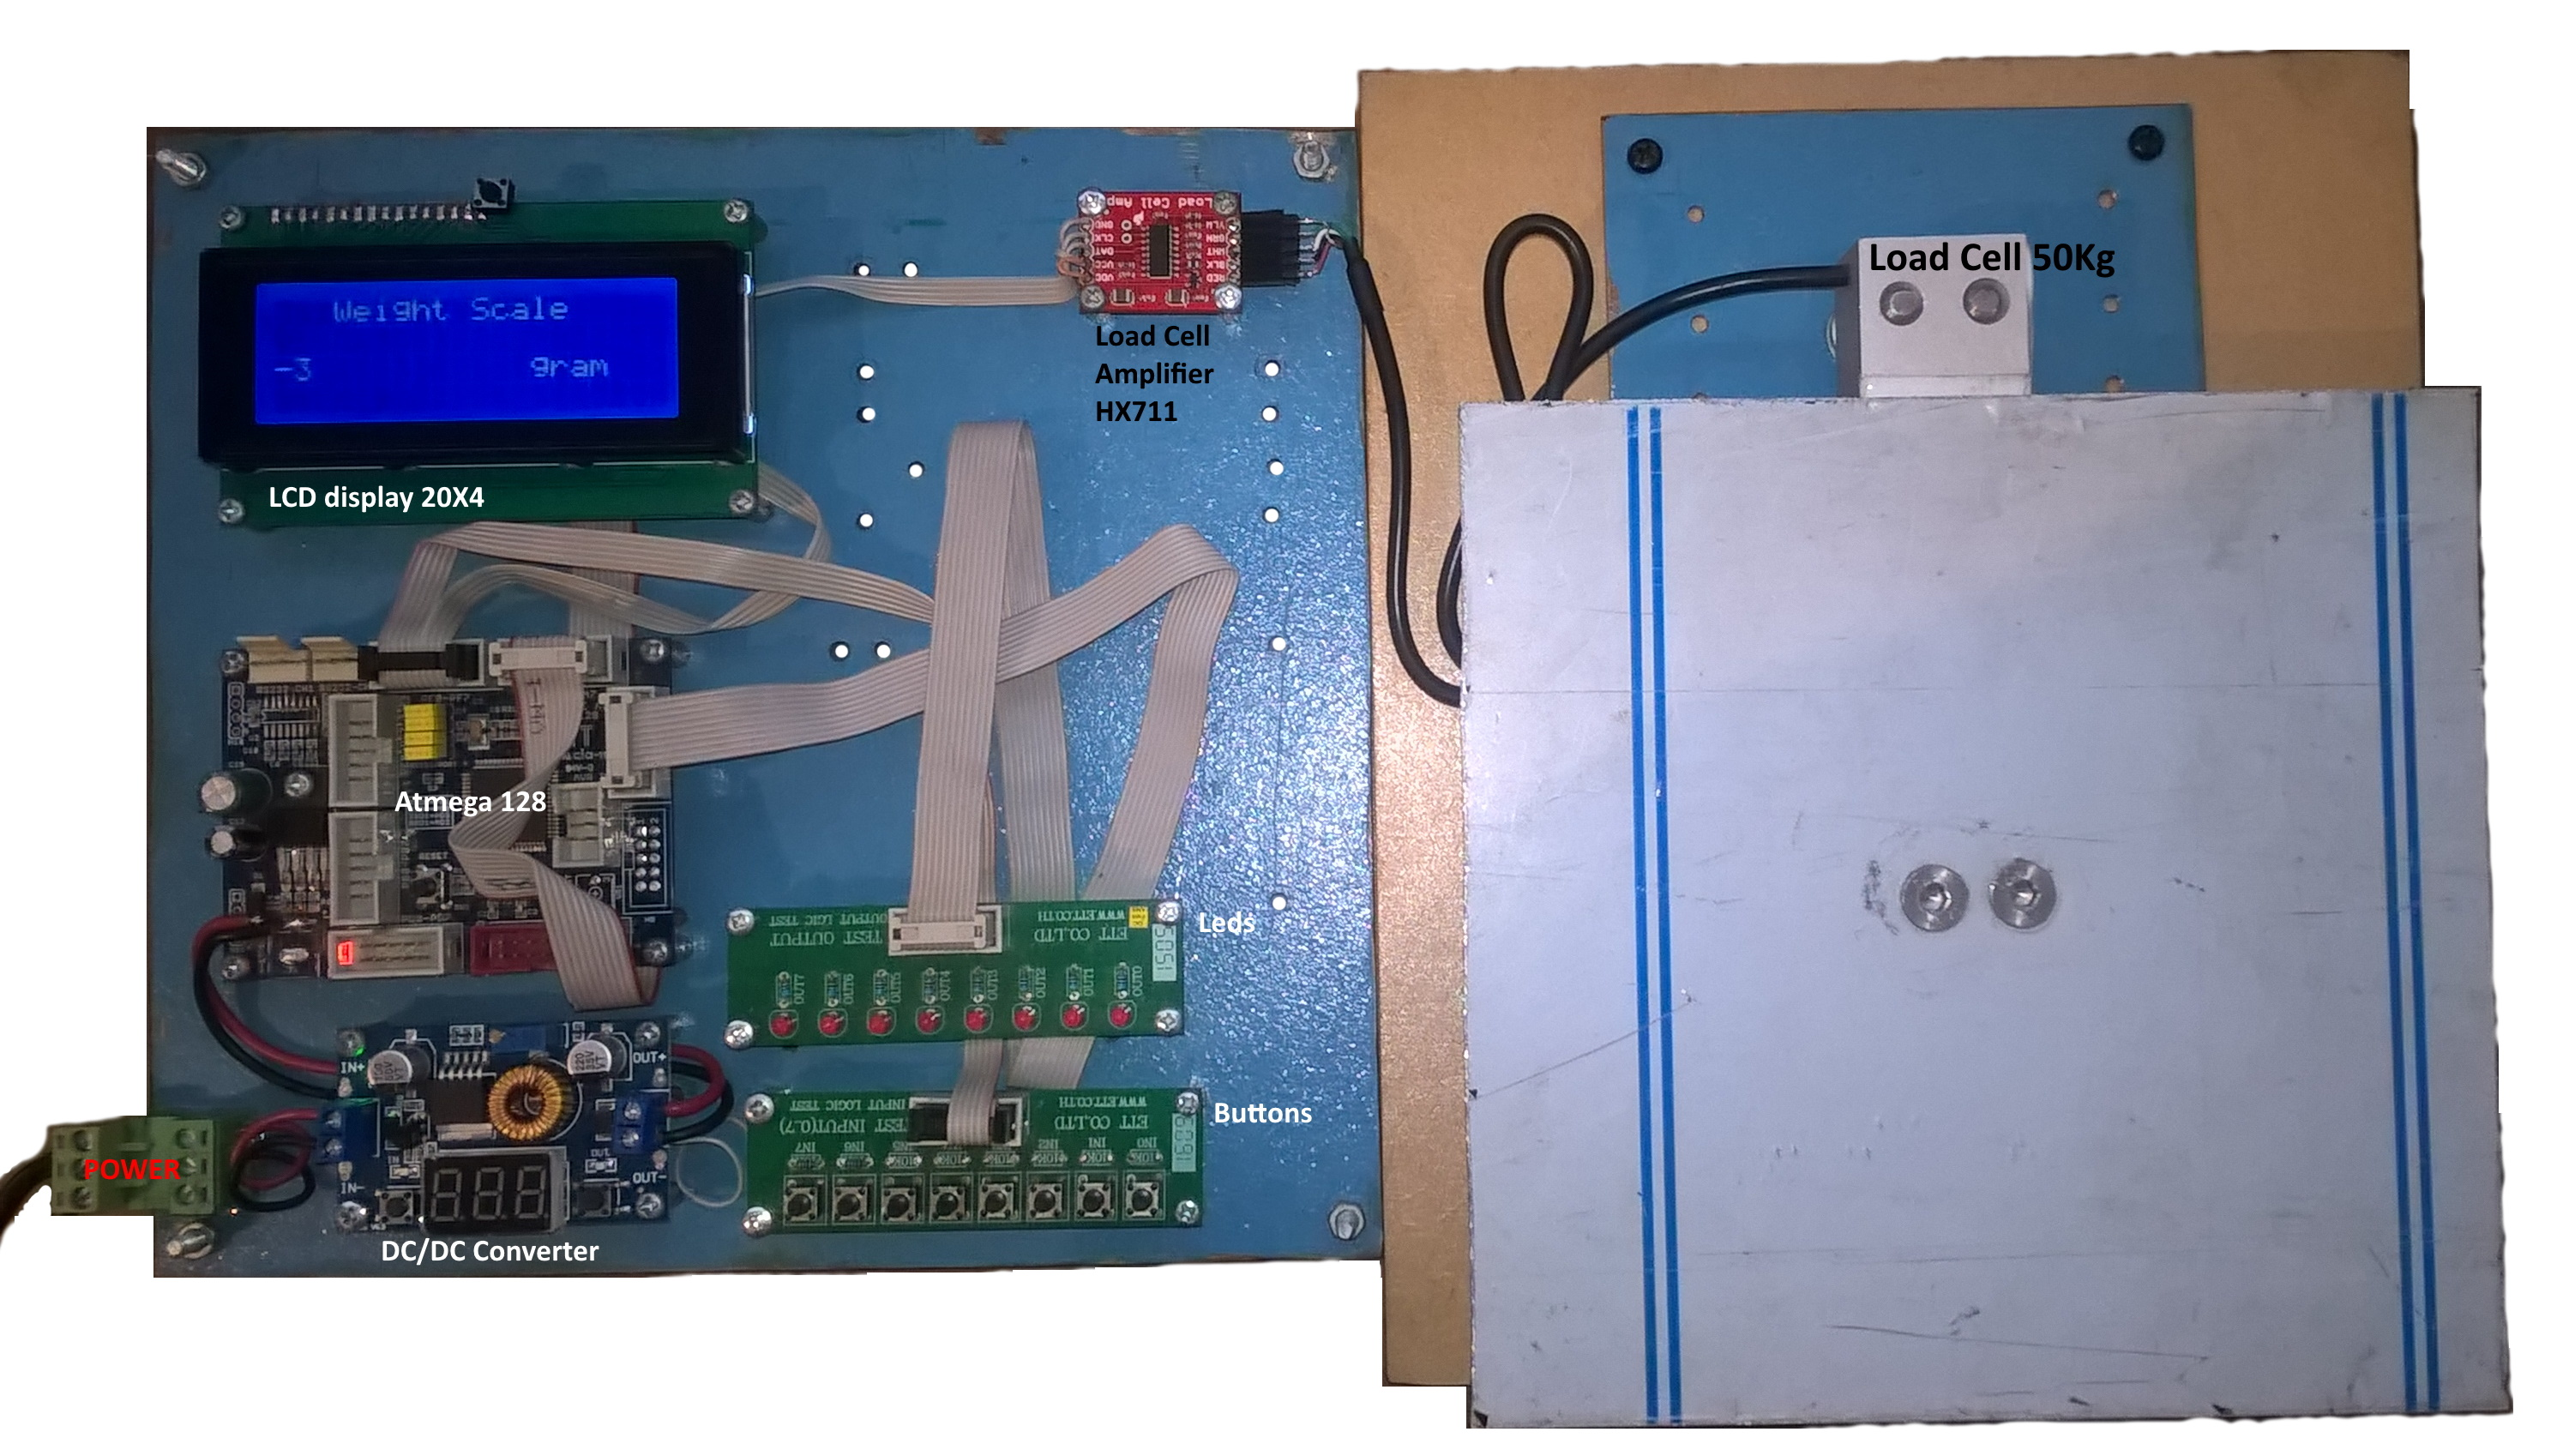
\includegraphics[scale=0.12]{./image/PESTA/kit/Kit_Desenvolvimento_2.jpg}
	\caption{Kit de Desenvolvimento}
	\label{Kit_Desenvolvimento_2}
\end{figure}
a seguir a \textit{figura} \ref{Block_diagram_1} representado os elementos em diagrama de blocos.
\begin{figure}[H]
	\centering
	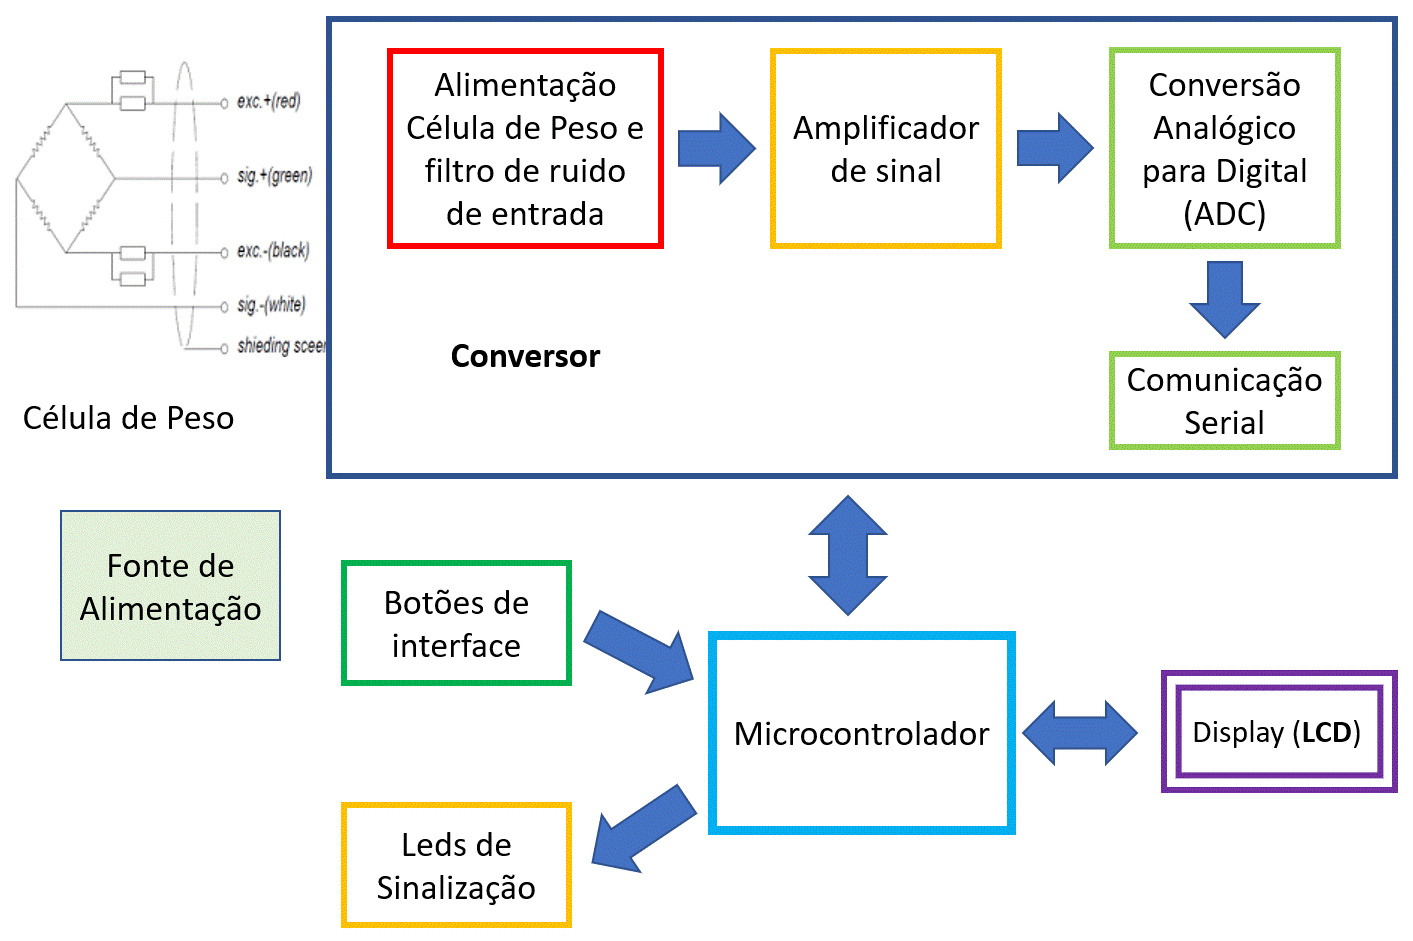
\includegraphics[scale=0.27]{./image/PESTA/Diagrama/Diagrama_bloco_3.jpg}
	\caption{Diagrama Blocos}
	\label{Block_diagram_1}
\end{figure}
\section{sensor}
Para medir a massa recorreu-se a uma \textbf{célula de peso} que determina a pressão exercida por um dado objeto, neste caso é um bloco de alumínio como indicado na \textit{figura} \ref{Load_Cell_1}, para isso ser possível este utiliza sensores Piezoresistivos numa montagem em ponte \textit{wheatstone} sobre essa superfície em locais determinados.
\\
\begin{figure}[H]
	\captionsetup{justification=raggedright,singlelinecheck=false}
	\flushleft
	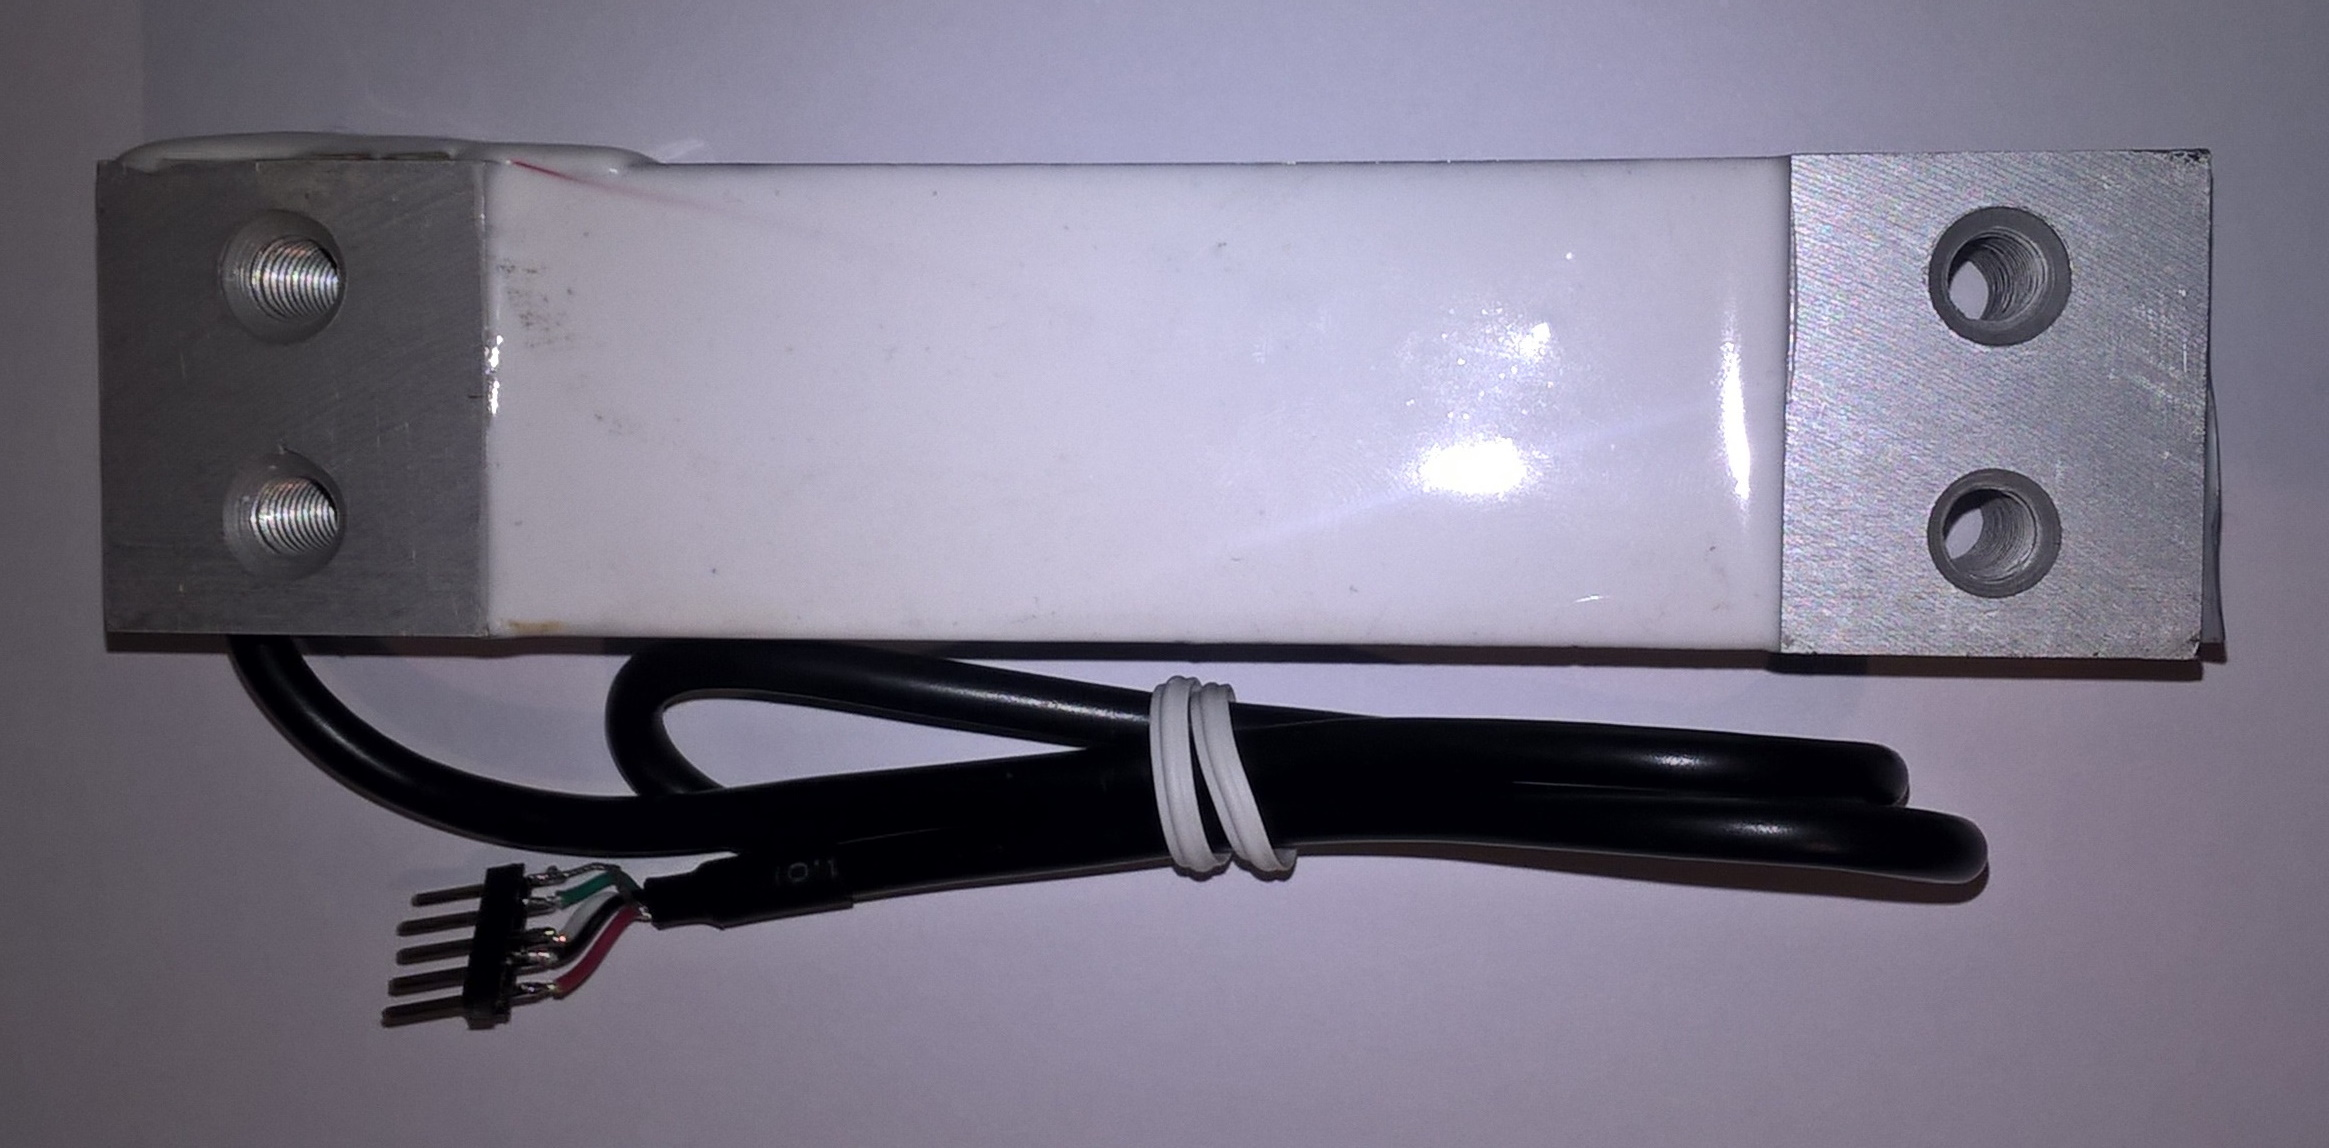
\includegraphics[scale=0.15]{./image/PESTA/material/Load_Cell_1.jpg}
	\caption{Célula de Peso 50Kg}
	\label{Load_Cell_1}
\end{figure}
\figurespace{.5}
Piezoresistividade deriva seu nome da palavra grega \textit{piezin}, que significa "pressionar". É um efeito exibido por vários materiais que exibem uma mudança na resistividade devido a uma pressão aplicada. O efeito foi descoberto pela primeira vez por Lord Kelvin em \textcolor{blue}{1856}, que notou que a resistência dos fios de cobre e ferro aumentava quando em tensão. Ele também observou que os fios de ferro apresentavam uma alteração maior na resistência do que os de cobre. A primeira aplicação do efeito piezoresistivo não apareceu até a década de \textcolor{blue}{1930}, cerca de \textcolor{blue}{75} anos após a descoberta de Lord Kelvin. Em vez de usar fios de metal, esses assim chamados medidores de tensão são geralmente feitos de uma folha de metal fina montada em uma película de suporte, que pode ser colada em uma superfície. O sensor de fita de metal típico é representado na \textit{figura} \ref{strain_gauge_1} \cite{book-9}.
\\
\\
\begin{minipage}[!b]{.5\linewidth}
\begin{figure}[H]
	\captionsetup{justification=raggedright,singlelinecheck=false}
	\flushleft
	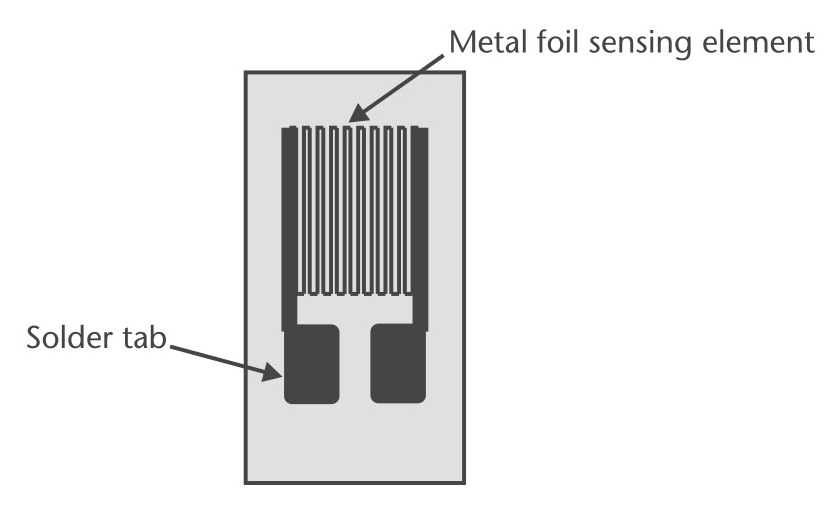
\includegraphics[height=5cm]{./image/PESTA/general/strain_gauge_1.jpg}
	\caption{Fita metálica \textit{strain gauge} \cite{book-9}}
	\label{strain_gauge_1}
\end{figure}
\end{minipage}
\begin{minipage}[!b]{.5\linewidth}
\begin{figure}[H]
	\captionsetup{justification=raggedright,singlelinecheck=false}
	\flushleft
	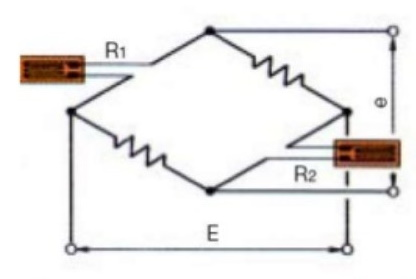
\includegraphics[height=5cm]{./image/PESTA/schematic/Wheatstone_2.jpg}
	\qquad \caption{Ponte \textit{Wheatstone}}
	\label{wheatstone_2}
\end{figure}
\end{minipage}
\minipagespace{.5}
\begin{minipage}[!b]{.4\linewidth}
	\begin{figure}[H]
		\captionsetup{justification=raggedright,singlelinecheck=false}
		\flushleft
		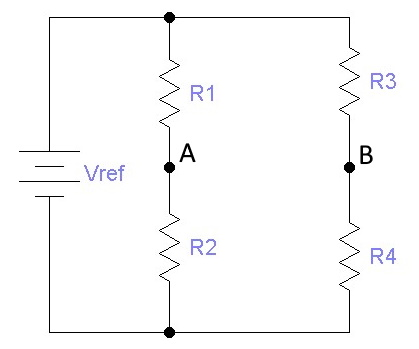
\includegraphics[height=5cm]{./image/PESTA/schematic/Wheatstone_1.jpg}
		\caption{\textit{Wheatstone} por resistências}
		\label{wheatstone_1}
	\end{figure}
\end{minipage}
\begin{minipage}[!b]{.6\linewidth}
	\begin{align}
		\label{eq:wheatstone}
		&V_A =  \frac{R_2}{R_1 + R_2} \; V_{ref} \; V_B=\frac{R_4}{R_3 + R_4} \; V_{ref} \\
		&V_{AB} =  V_A - V_B = e \\
		&V_{AB}= \left(\frac{R_2}{R_1 + R_2} - \frac{R_4}{R_3 + R_4}\right) \; Vref \\
		&e = \frac{R_2 R_3 - R_4 R_1}{(R_1 + R_2)(R_3 + R_4)} \; Vref
	\end{align}
	\minipagespace{.1}
\end{minipage}
\minipagespace{.5}
Normalmente nestas aplicações só é usados um sensor ou dois sensores em que estão nos extremos opostos  ou ligados ao mesmo ponto da alimentação, só em casos muito raros são utilizados os quatro sensores na qual a sensibilidade é máxima. E como é óbvio se o valor das quatro resistências são iguais $V_{AB}$ na saída é nula, e quando se utiliza apenas dois sensores a sensibilidade do sistema é intermédia.
\newpage
A montagem da mesa de medição \textit{figura} \ref{Prato},
\minipagespace{5}
\begin{minipage}[!b]{\linewidth}
\begin{figure}[H]
	\centering
	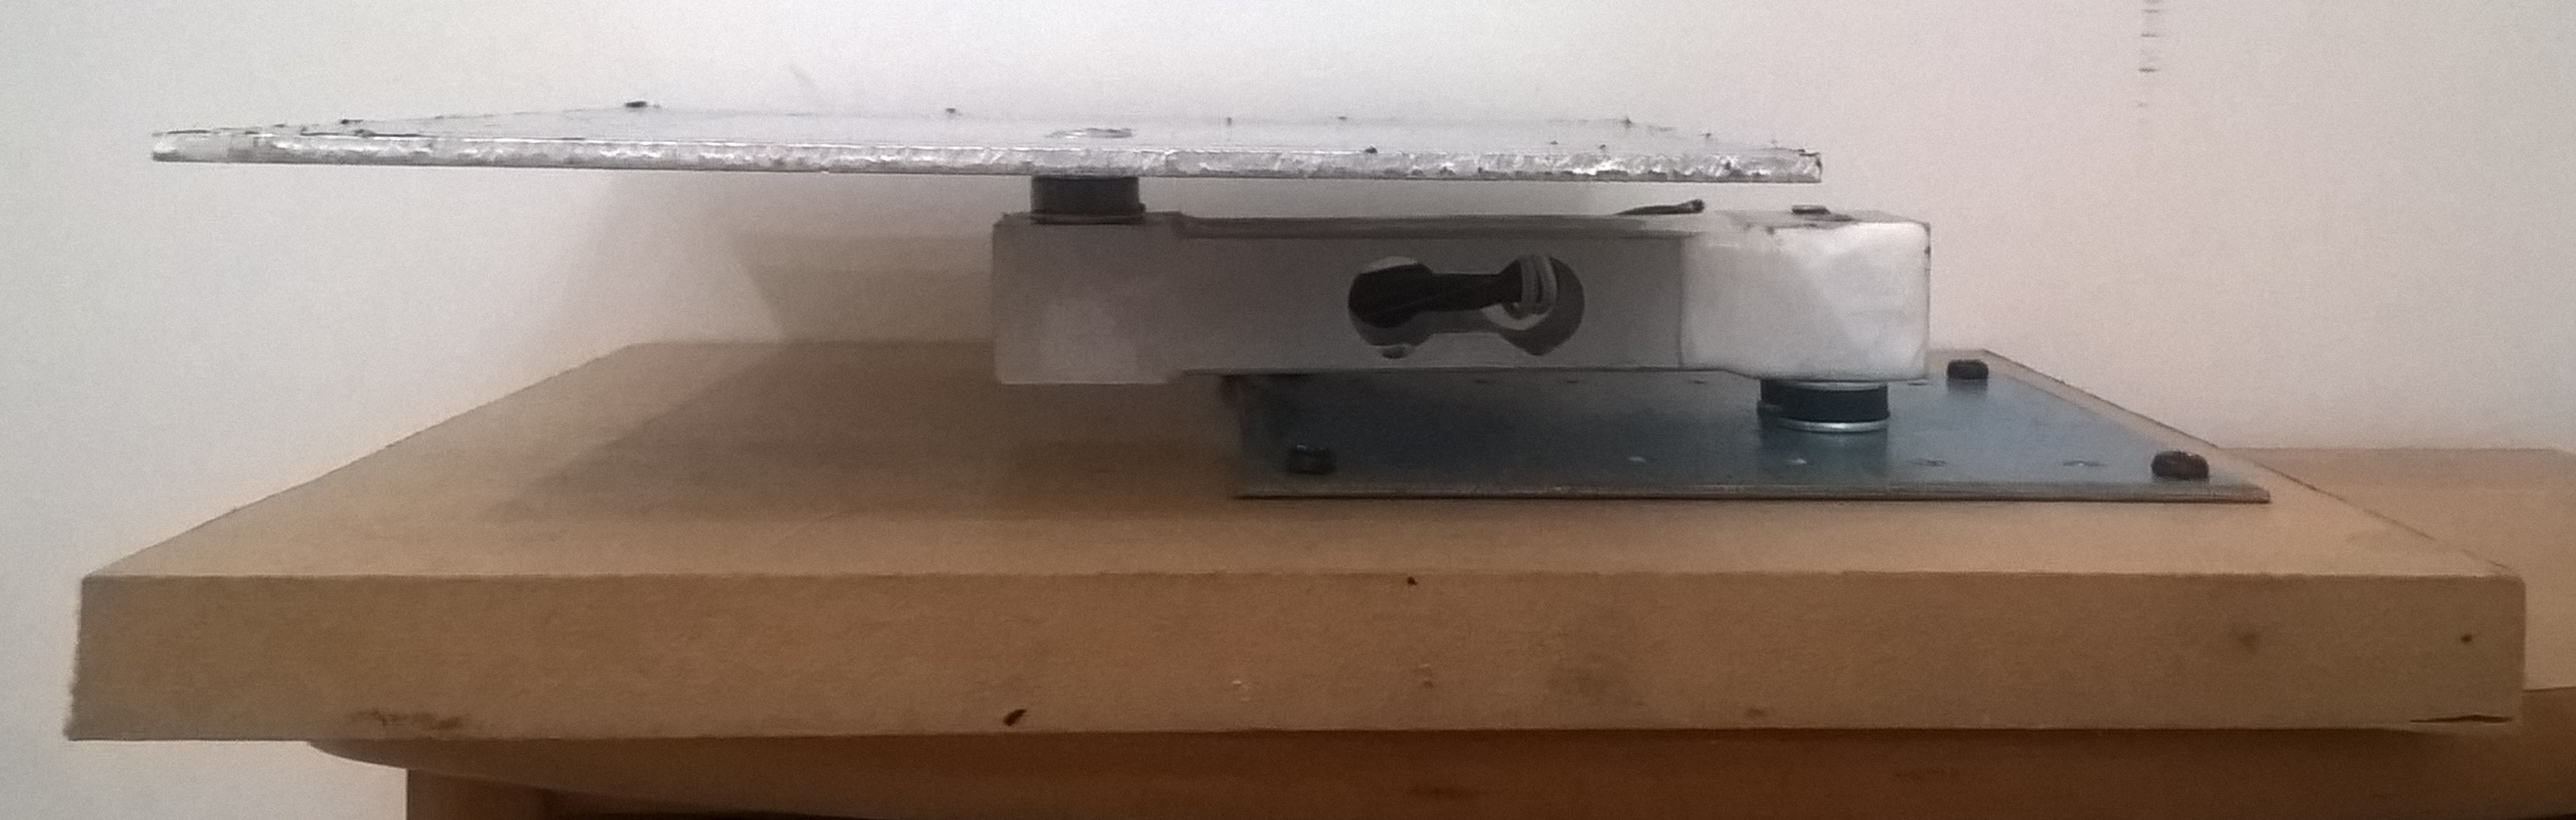
\includegraphics[scale=0.16]{./image/PESTA/material/Prato.jpg}
	\caption{Prato}
	\label{Prato}
\end{figure}
\end{minipage}
\newpage
\section{Amplificador de sinal}
A amplificação é geralmente um requisito fundamental, pois a maioria dos sensores tende a produzir níveis de sinal significativamente mais baixos do que aqueles usados no processador digital. Sensores resistivos podem precisar de um amplificador de carga. Se possível, é vantajoso ter o ganho o mais próximo possível do elemento sensor. Em situações onde um alto ganho é necessário, muitas vezes pode haver implicações para lidar 
com quaisquer efeitos adversos, como o ruído, também em termos de \textit{layout} do \textit{chip}, os transitórios agudos associados aos sinais digitais precisam ser mantidos bem longe dos circuitos analógicos \textit{front-end}. \cite{book-9}
\\
\\
A ligação destes componentes é intuitivo e fácil de se perceber, o que é complexo neste trabalho é a interligação destes equipamentos com o micro-controlador por meio de \textit{software} e criar o \textit{driver} de comunicação para a placa do amplificador de sinal, já que o protocolo de comunicação é proprietário.
\\
\\
\begin{figure}[H]
	\captionsetup{justification=raggedright,singlelinecheck=false}
	\centering
	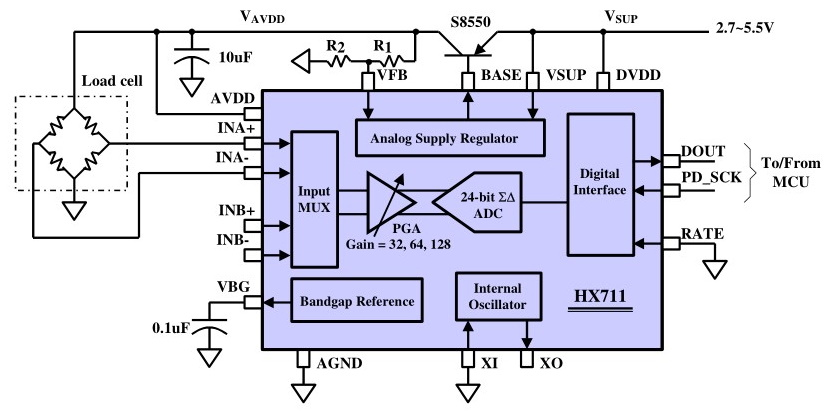
\includegraphics[scale=0.35]{./image/PESTA/schematic/HX711_Schematic_1.jpg}
	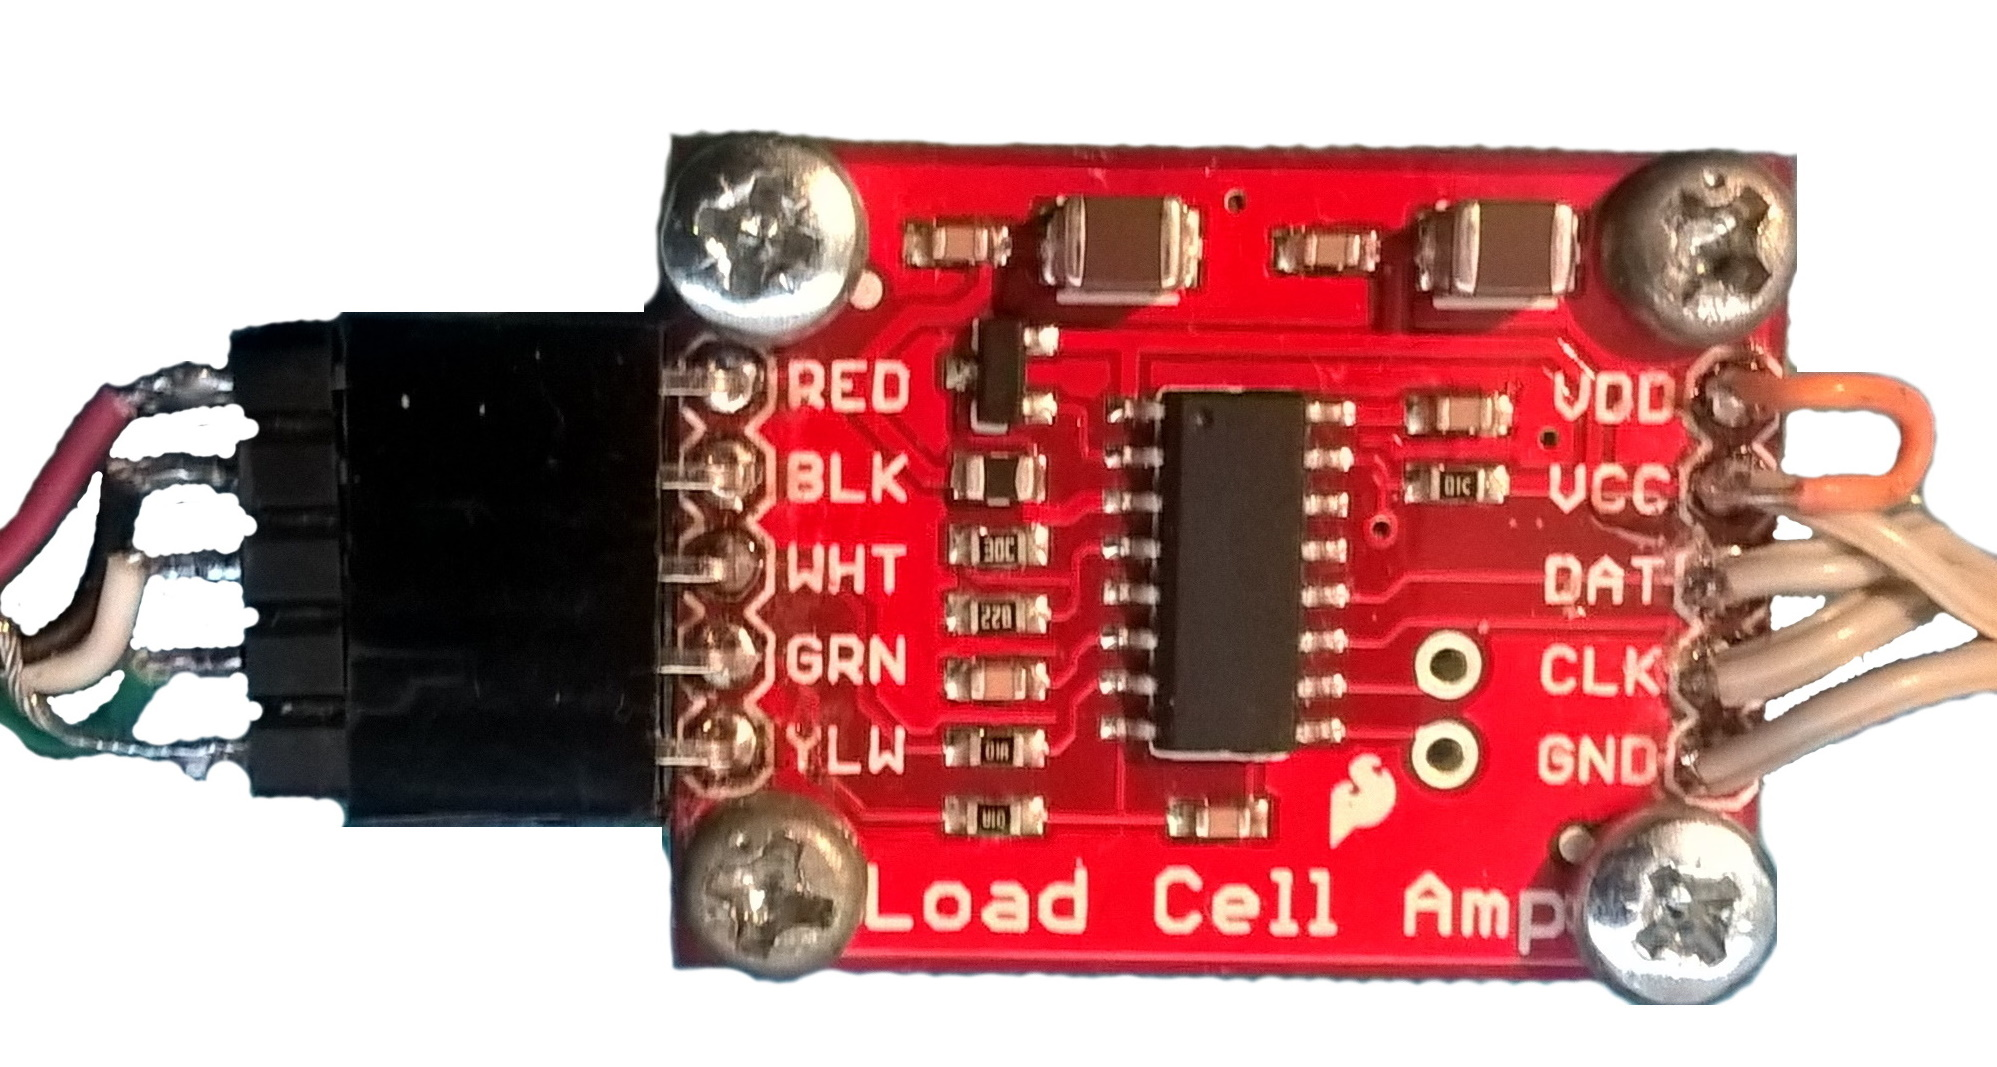
\includegraphics[scale=0.1]{./image/PESTA/material/HX711_board_1.jpg}
	\caption{Amplificador de Sinal [HX711]}
	\label{HX711_Schematic_1}
\end{figure}
\figurespace{.5}
A placa \textit{Load Cell Amplifier }pode ser programada fisicamente para determinar o numero de amostras por segundo a ser transmitido, tem opção de \textcolor{blue}{10} amostras por segundo e \textcolor{blue}{80} amostras, neste projeto optei pela segunda opção que necessita alteração na placa de circuito de impresso, isto é, abrir o \textit{jumper} respetivo de configuração.
\\
\\
\begin{table}[H]
	\centering
	\caption{Terminais HX711 ({\tiny \scriptsize{top view}})}
	\begin{tabular}{||L{1cm} C{3cm} | p{3cm}  C{2cm}||}
		\hline
		\multicolumn{2}{||c|}{MCU} & \multicolumn{2}{|c||}{\textit{Célula de peso}}\\ [1ex]
		\hline
		1 & GND & EARTH (GND) & YLW \\ 
		2 & CLK & INPA & GRN \\
		3 & DATA & INNA & WHT \\
		4 & VCC &  GND & BLK \\
		5 & VDD & $V_{ADC}$ & RED \\ [1ex]
		\hline
	\end{tabular}	
	\label{HX711_connection}
\end{table}
\tablespace{.5}
A conversão de informação é a transição entre o sinal continuo da vida real para um sinal discreto associado ao mundo digital, tipicamente esta etapa consiste na conversão analógica para digital.
\\
O processamento digital pode consistir de rotinas para compensar os desvios por linearização, compensação da sensibilidade e \textit{offset}, ou podem ser técnicas mais sofisticadas como reconhecimento de padrões (tais como redes neuronais) para equipamentos de sensores vetoriais.\cite{book-9}
\\
A comunicação trata de cuidar das rotinas necessárias para transferir e receber a informação e sinais de controle para a linha de comunicação com o sensor, e o processador que toma lugar como componente central tratando a informação, guardar os dados e fazer rotinas tais como de calibração, teste e controlo de ganho da amplificação. \cite{book-9}
\\
\\
\begin{figure}[H]
	\centering
	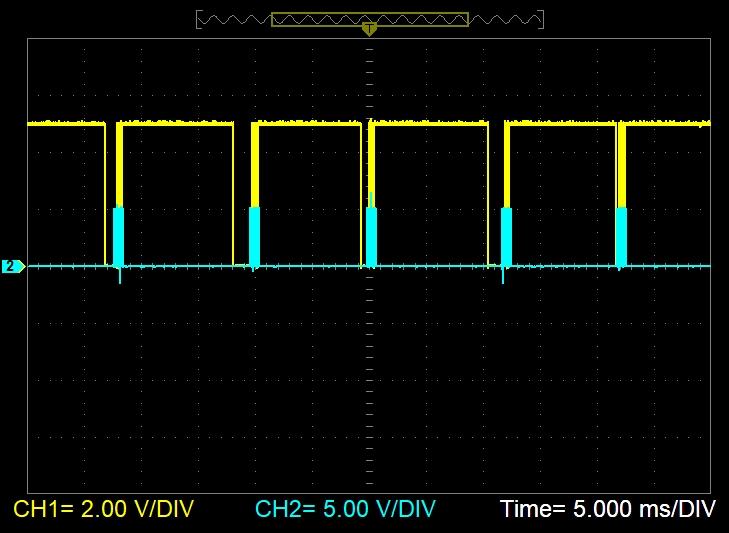
\includegraphics[scale=0.55]{./image/PESTA/graph/80SPS64GAIN/SPS_80.JPG}
	\caption{Amostras}
	\label{SPS_64}
\end{figure}
\figurespace{.5}
A livraria (\textit{driver}) criada recorre a interrupções periódicas quando o sinal de \textit{data} vai para a massa, indicando assim que tem um pacote de leitura pronto a ser transmitido.
\\
\\
\begin{minipage}[!b]{.40\linewidth}
	\begin{table}[H]
		\captionsetup{justification=raggedright,singlelinecheck=false}
		\caption{Configuração Ganho}
		\begin{tabular}{ | c | c | c |  }
			\hline
			\makecell[c]{PD\_SCK \\ Impulsos} & Entrada  & Ganho \\
			\hline
			\hline
			25 & \textbf{A} & 128 \\
			\hline
			26 & \textbf{B} & 32 \\
			\hline
			27 & \textbf{A} & 64 \\
			\hline
		\end{tabular}
		\label{Gain_Selection}
	\end{table}
	\tablespace{2}
\end{minipage}
\begin{minipage}[l]{.6\linewidth}
\vspace{.3cm}
Como indicado abaixo no gráfico em que a linha \textcolor{yellow}{amarela} é a informação e a linha \textcolor{BlueGreen}{azul} o respetivo \textit{clock} que é gerado pelas interrupções do micro-controlador fazendo \textit{shift} dos \textcolor{blue}{24} bits, que depois no fim transmite para o amplificador o ganho de amplificação a ser usado pelo numero excedente de \textit{clock cycles}, em que nesta demonstração \textit{figura} \ref{Gain_128_example} é \textcolor{blue}{um}, e corresponde a ganho de \textcolor{blue}{128}, respeitando a \textit{tabela} \ref{Gain_Selection},  e a sequir o exemplo da \textit{figura} \ref{Gain_64_example} com o ganho de \textcolor{blue}{64}, pois tem \textcolor{blue}{três} impulsos excedentes.
\\
\end{minipage}
\minipagespace{.5}
\begin{minipage}[!b]{.5\linewidth}
\begin{figure}[H]
	\captionsetup{justification=raggedright,singlelinecheck=false}
	\flushleft
	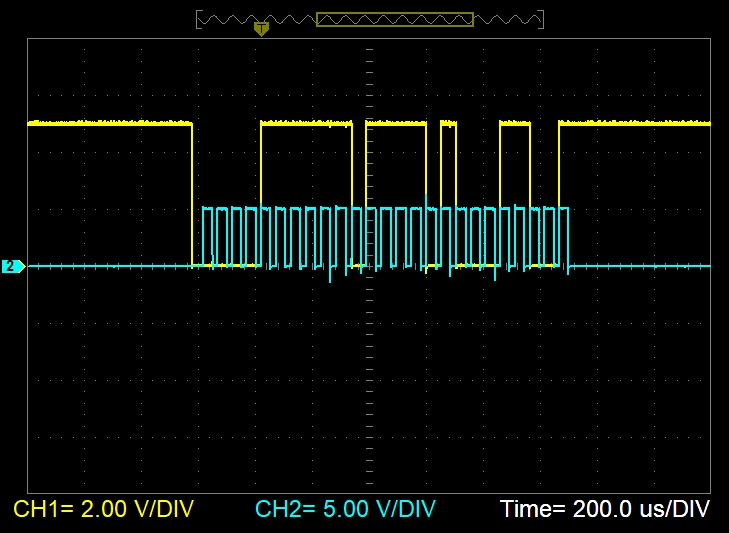
\includegraphics[scale=0.25]{./image/PESTA/graph/80SPS128GAIN/Gain_128_example.JPG}
	\caption{Ganho de 128}
	\label{Gain_128_example}
\end{figure}
\end{minipage}
\hspace{1cm}
\begin{minipage}[!b]{.5\linewidth}
\begin{figure}[H]
	\captionsetup{justification=raggedright,singlelinecheck=false}
	\flushleft
	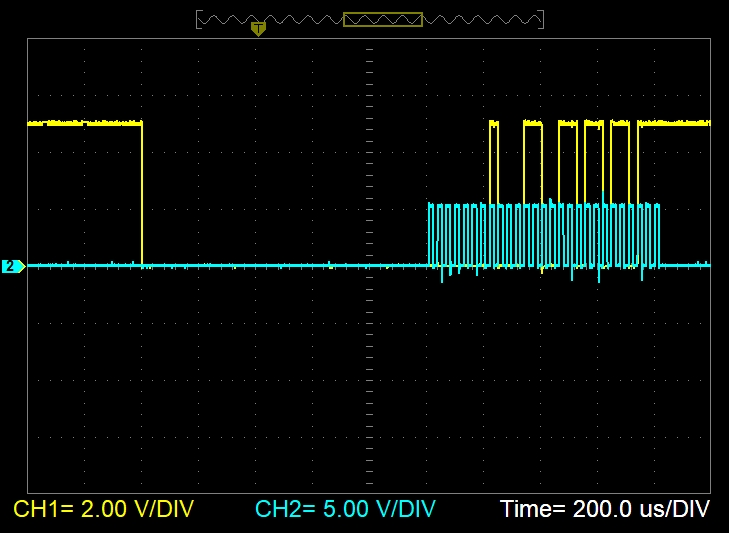
\includegraphics[scale=0.25]{./image/PESTA/graph/80SPS64GAIN/Gain_64_example.JPG}
	\caption{Ganho de 64}
	\label{Gain_64_example}
\end{figure}
\end{minipage}
\minipagespace{.5}
Para obter este resultado a livraria driver para o \textit{Load Cell Amplifier} teve de ter em consideração que o microcontrolador é de \textcolor{blue}{8} bits, porque o pacote de informação consiste de \textcolor{blue}{24} \textit{bits} e em que é transmitido primeiro o \textit{bit} \textbf{MSB}.
\\
\\
\\
O código que executa esta rotina é demonstrado na \textit{lista} \ref{HX711-read-raw} que é chamada pelas interrupções periódicas e só é ativa quando a função na \textit{lista} \ref{Main-While-case-1} \textbf{hx.query(\&hx)} é verdadeira.
\\
\\
{ \tiny
	\lstinputlisting[language=C, caption={função de chamada \textbf{hx.query(\&hx)}}, captionpos=b, label=Main-While-case-1]{./input/code/Main_While_case_1.c}
}
\newpage
{ \tiny
	\lstinputlisting[language=C, caption=HX711\_read\_raw, captionpos=b, label=HX711-read-raw]{./input/code/HX711_read_raw.c}
}
\begin{comment}
\begin{minipage}[l]{\linewidth}
\begin{minipage}[l]{.60\linewidth}
\begin{figure}[H]
	\flushleft
	\captionsetup{justification=raggedright,singlelinecheck=false}
	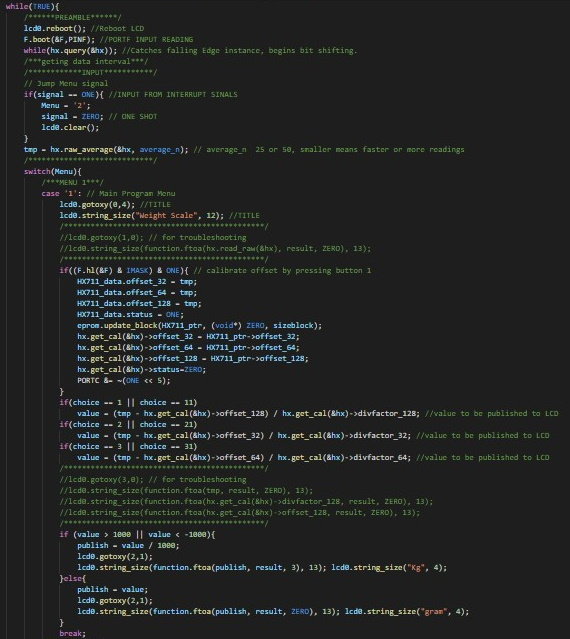
\includegraphics[scale=0.55]{./image/PESTA/Code/Main_While_Balanca.jpg}
	\caption{PROGRAM 1}
	\label{Main_While_Balanca}
\end{figure}
\end{minipage}
\begin{minipage}[l]{.33\linewidth}
	\vspace{1.1cm}
	\begin{figure}[H]
		\flushleft
		\captionsetup{justification=raggedright,singlelinecheck=false}
		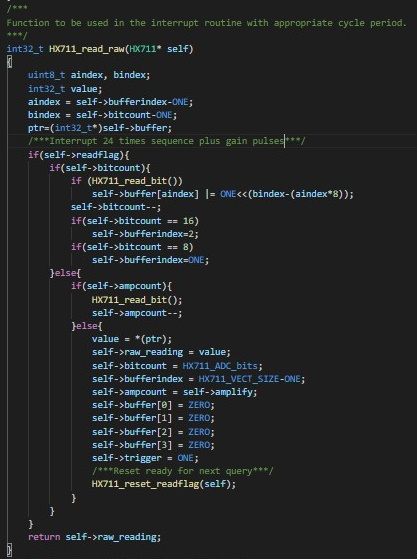
\includegraphics[scale=0.55]{./image/PESTA/Code/read_raw.jpg}
		\caption{Leitura ADC}
		\label{read_raw}
	\end{figure}
\end{minipage}
\end{minipage}
\minipagespace{.5}
\end{comment}
\listingspace{.5}
Após obter um numero determinado de valores discretos é calculado sua média
\begin{equation}
	\label{eq:Mean}
	\overline{x}  =  \frac{1}{n}\sum_{i=1}^n x_i
\end{equation}
para ser tratado e deduzido o valor correspondente da massa.
\newpage
\section{Display LCD}
O \textit{Liquid-Crystal Dispaly} (\textbf{LCD}) utilizado é de 4x20, isto é, quatro linhas de vinte caracteres cada, é o interface humano principal, e durante o projecto uma ferramenta extremamente útil também para fazer \textit{debug} e executar testes no código.
\\
\\
Uma livraria na qual já tinha feito para outros projetos serviu para aplicar neste, poupando bastante tempo, revelando a importância de documentar os conhecimentos adquiridos. A livraria ou se preferem \textit{driver} esta \textit{anexado}.
%[\ref{codigo}]
\\
\\
Abaixo esta uma tabela \ref{LCD_connections} com as respetivas ligações.
\tablespace{.2}
\begin{table}[H]
	\centering
	\caption{Conexões \textbf{LCD}}
	\begin{tabular}{||p{1cm} p{2cm} p{4cm} | p{1cm}||} 
		\hline
		\multicolumn{3}{||c|}{\textbf{LCD Pin}} & \multicolumn{1}{|c||}{\textbf{MCU Pin}}\\ [1ex]
		\hline
		1 & VSS & GND & \\
		2 & VCC & +5V & \\
		3 & VEE & \textit{Contrast Control} & \\
		4 & RS & \textit{Register Select} & Pin 0 \\
		5 & RW & \textit{Read/Write} & Pin 1 \\
		6 & E & \textit{Enable} & Pin 2 \\
		7 & Do & \textit{Data Pin 0} & \\
		8 & D1 & \textit{Data Pin 1} & \\
		9 & D2 & \textit{Data Pin 2} & \\
		10 & D3 & \textit{Data Pin 3} & \\
		11 & D4 & \textit{Data Pin 4} & Pin 4 \\
		12 & D5 & \textit{Data Pin 5} & Pin 5 \\
		13 & D6 & \textit{Data Pin 6} & Pin 6 \\
		14 & D7 & \textit{Data Pin 7} & Pin 7 \\
		15 & LED+ & \textit{Led +5V} &  \\
		16 & LED- & \textit{Led Ground} & \\
		\multicolumn{3}{||c|}{\textit{Reboot} LCD} & \multicolumn{1}{|l||}{Pin 3}\\ [1ex]
		\hline
	\end{tabular}	
	\label{LCD_connections}
\end{table}
\begin{figure}[H]
	\centering
	%%\captionsetup{justification=raggedright,singlelinecheck=false}
	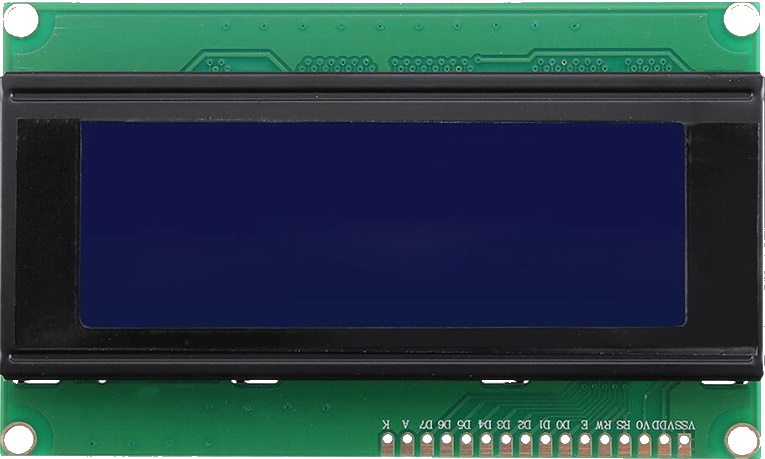
\includegraphics[scale=.5]{./image/PESTA/material/4x20_LCD.jpg}
	\caption{LCD}
	\label{4x20_LCD}
\end{figure}
\newpage
\section{Micro-controlador}
Os microcontroldores da \textbf{Atmel} de 8 e 32 bits são baseados na arquitetura avançada de \textbf{Harvard} na qual esta concebido para baixos consumos e performance.
\\
\\
Este tipo de arquitetura tem dois  \textit{busses} (barramentos) um dedicado a leitura das instruções a executar e outra para escrita e leitura de \textit{data} (informação ou dados), isto assegura que uma nova instrução pode ser executada em cada ciclo de relógio, na qual elimina estados de espera quando não ha instruções prontas a executar.
\\
\\
Nos microcontroladores da \textbf{AVR} os barramentos estão configurados de forma a dar prioridade ao barramento das instruções do \textbf{CPU} acesso a memoria flash enquanto o barramento da CPU de dados tem prioridade de acesso a \textbf{SRAM} (Static Random Access Memory).
\\
\\
O espaço de memoria de dados é dividida em três, os \textbf{GPR} (General Purpose Registers) as \textbf{SFRs} (Special Function Registers) ou memoria de I/O e a \textit{data} \textbf{SRAM}.
\\
\\
Os microcontroladores da \textbf{AVR} utiliza uma arquitetura de instruçõeses \textbf{RISC} (Reduced Instruction Set Computer ou Reduced COMPLEXITY Instruction Set Computer) na qual reduz a complexidade dos circuitos na codificação de cada instrução.
\\
\\
Dai que os microcontroladores que se baseiam nestes tipos de arquitetura são sinonimo de código reduzido, alta performance e baixo consumo energético.
\\
\\
\begin{figure}[H]
	\centering
	%%\captionsetup{justification=raggedright,singlelinecheck=false}
	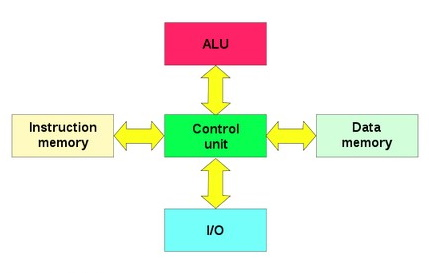
\includegraphics[scale=1]{./image/PESTA/Diagrama/Harvard_architecture.jpg}
	\caption{Harvard Architecture}
	\label{Harvard_architecture}
\end{figure}
\qquad link: \url{https://en.wikipedia.org/wiki/Harvard_architecture}
\newpage
Neste projeto apostei no Atmega 128 (\textit{figura} \ref{Atmega_128_pinagem}) por ser um dos mais poderosos \textbf{MCU´s} da linha de 8 b\textit{bit} da Atmel, também por estar integrado já numa placa de desenvolvimento usando o sistema por fichas \textit{insulation-displacement contact} (\textbf{IDC}) que prefiro, ou seja, usando \textit{flatcables} para ligar os periféricos, e considero muito mais pratico do que sistema que esta na moda, tais como a linha Arduino e da STM por ter um interface por pinos.
\\
\\
\\
\\
\\
\begin{figure}[H]
	\centering
	%%\captionsetup{justification=raggedright,singlelinecheck=false}
	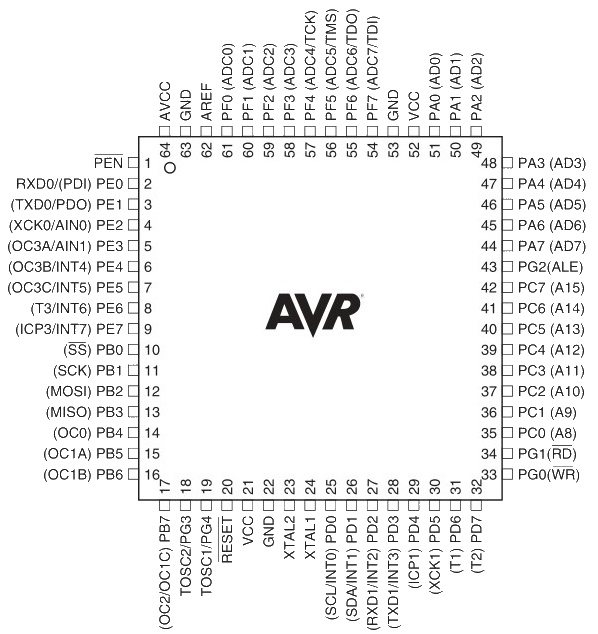
\includegraphics[scale=0.7]{./image/PESTA/material/Atmega128_1.jpg}
	\caption{Atmega 128}
	\label{Atmega_128_pinagem}
\end{figure}
\figurespace{1}
{Transparências Sistemas Digitais 2 \quad \textbf{ISEP} \quad 2008/2009 \quad \textit{link}}:
\\
\url{https://drive.google.com/file/d/1wgOGf8WwYY0OzDhRca9ypXz-iBO55YOF/view?usp=sharing}
\newpage
A características do micro-controlador ATmega 128 esta abaixo indicados na lista, os temporizadores considero o mais importante, o ADC nem vai ser usado neste projeto a alternativa é muito melhor, talvez os MCU nem deviam ter esta funcionalidade e realçar em meios de comunicação e memoria com as livrarias já disponíveis, este integrado é perfeito para esta aplicação em causa, sempre que fazemos projetos também temos de considerar os MCU de 32 \textit{bit} mas existe uma linha muito fina de apostar noutra alternativa e trabalhar com um sistema operativo devido a complexidade exigida, muito mais configurações e opções disponíveis do que um micro-controlador de 8 e 16 \textit{bit}.
\\
\\
\\
\begin{minipage}{\linewidth}
{\Large Caracteristicas do Atmega 128 :}
\begin{itemize}	
	\setlength\itemsep{-0.3em}
	\item Arquitectura RISC
	\item 33 instruções (a maior parte executada num único ciclo de execução)
	\item 32 x 8 registos de trabalho (arquitectura de registos)
	\item Até 16 MIPS (@16MHz) – 62.5ns / instrução
	\item 64K x 16 palavras de programa – 128K bytes FLASH
	\item 4K bytes de RAM interna
	\item 4K bytes de E2PROM de dados
	\item Ciclos de escrita / leitura – FLASH=10000, E2PROM=100000
	\item 7 Portos de IO \\
		\hspace*{.5cm}	-> 6 x 8 bits (Portos A .. F) \\
		\hspace*{.5cm}	-> 1 x 5 bits (Porto G)
	\item 2 x Timer / Counter de 8 bits
	\item 2 x Timer / Counter de 16 bits
	\item 1 x Real Time Counter ( com oscilador independente)
	\item 2 x PWM de 8 bits
	\item 6 x PWM de 16 bits
	\item ADC de 10 bits (8 canais)
	\item 2 x USART
	\item SPI
	\item TWI (I2C)
\end{itemize}
\end{minipage}
\minipagespace{0.5}
\newpage
Para programar este microcontrolador (\textbf{Atmega 128}) foi utilizado o programador da marca da Atmel precisamente o \textbf{Atmel-ICE} \textit{figura} \ref{Programador_1}, que para este equipamento tem disponível programação via \textit{In-System Programming} (\textbf{ISP}) \textit{figura} \ref{ISP_6_8_10pin} e \textit{Joint Test Action Group} (\textbf{JTAG}).
\minipagespace{.2}
\begin{minipage}[!b]{.5\linewidth}
	\begin{figure}[H]
		\captionsetup{justification=raggedright,singlelinecheck=false}
		\flushleft
		\includegraphics[scale=0.75]{./image/PESTA/programador/Atmel_ice.png}
		\caption{Diagrama Blocos}
		\label{Programador_1}
	\end{figure}
\end{minipage}
\hspace{.5cm}
\begin{minipage}[!b]{.5\linewidth}
	\begin{figure}[H]
		\captionsetup{justification=raggedright,singlelinecheck=false}
		\flushleft
		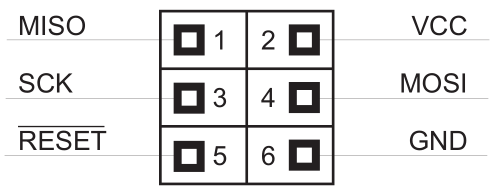
\includegraphics[scale=0.45]{./image/PESTA/programador/isp_6pin.png}
		\hspace{.3cm}
		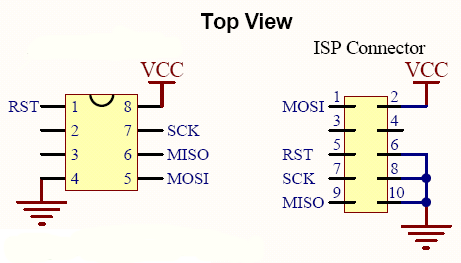
\includegraphics[scale=0.5]{./image/PESTA/programador/isp_8e10pin.png}
		\caption{Fichas \textbf{ISP}}
		\label{ISP_6_8_10pin}
	\end{figure}
\end{minipage}
\chapter{Software}
O \textbf{IDE} utilizado neste trabalho foi o \textbf{\textit{{Microchip Studio for AVR\textsuperscript{\textregistered} and SAM Devices}}} (\textit{version: 7.0.2542}). A programação foi feita em Linguagem \textbf{C}, sua estrutura sintática esta abaixo mencionado:
\\
\\
\begin{figure}[H]
	\centering
	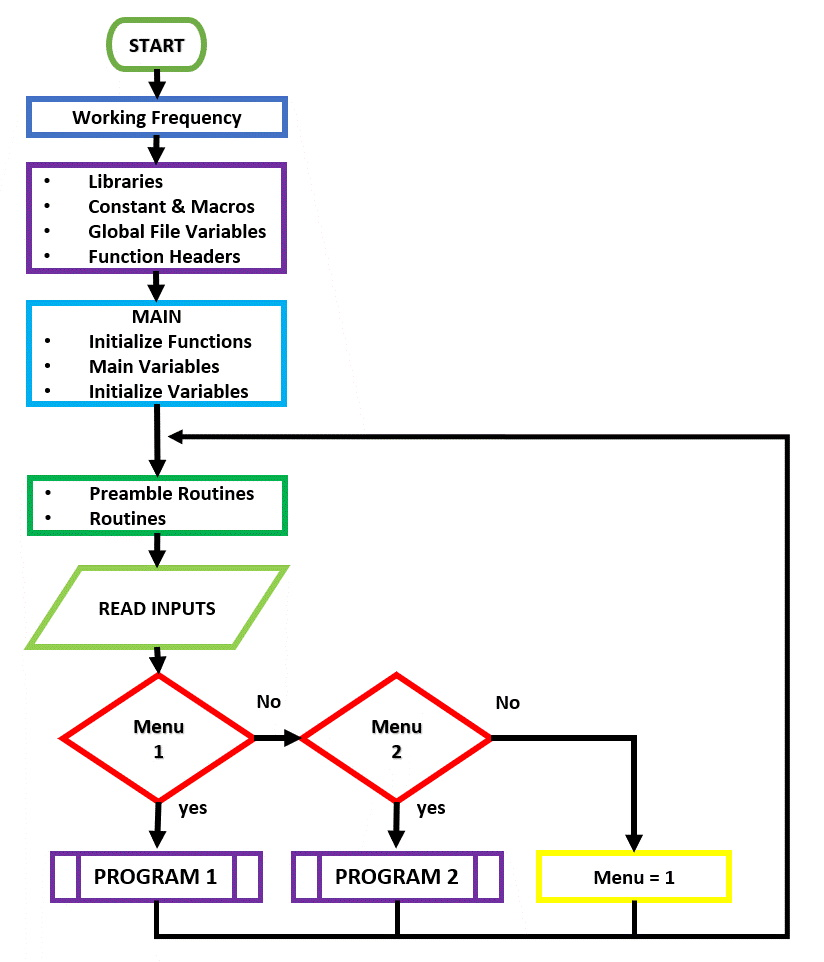
\includegraphics[scale=0.6]{./image/PESTA/flowchart/Main_Program_1.jpg}
	\caption{Estrutura do Programa}
	\label{Main_Program_1}
\end{figure}
\figurespace{.5}
O \textit{PROGRAM 1} é onde corre o programa da balança, e o \textit{PROGRAM 2} usado para calibração do \textit{Gain Factor}.
\\
\\
Todos os programas sequem uma estrutura sintática recursiva usando o seguinte modelo.
\\
\\
\begin{figure}[H]
	\centering
	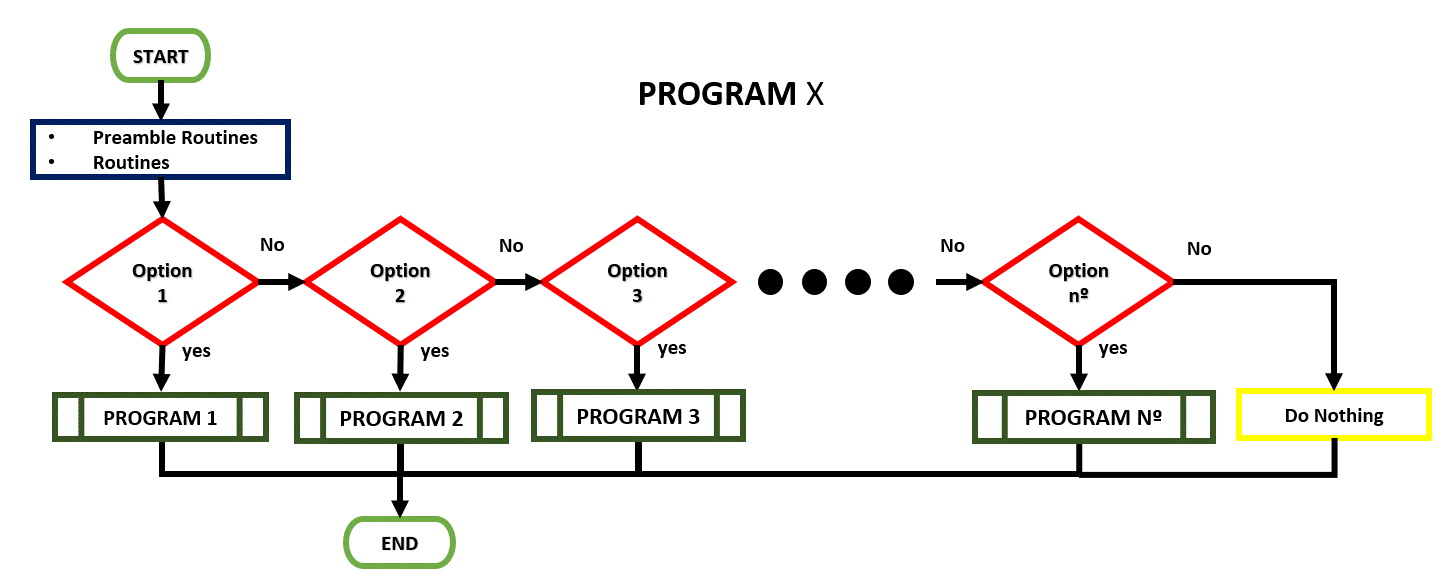
\includegraphics[scale=0.40]{./image/PESTA/flowchart/Generic_structure.jpg}
	\caption{Sintaxe Genérica dos programas}
	\label{Geneic_structure}
\end{figure}
\figurespace{.5}
Duas interrupções periódicas estão sempre a correr em \textit{background}, uma para fazer o \textit{shift} dos \textit{bit´s} da conversão \textbf{ADC} feita pelo amplificador de sinal HX711 e outra interrupção periódica de segundo em segundo usado para saltar de \textit{Menu} pelos botões.
\\
\\
\begin{minipage}{\linewidth}
\begin{minipage}{.5\linewidth}
\begin{figure}[H]
	\centering
	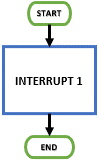
\includegraphics[scale=0.7]{./image/PESTA/flowchart/Interrupt_1.jpg}
	\caption{\textbf{ADC} conversão}
	\label{Interrupt_1}
\end{figure}
\end{minipage}
\begin{minipage}{.5\linewidth}
\begin{figure}[H]
	\centering
	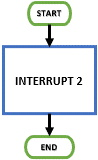
\includegraphics[scale=0.7]{./image/PESTA/flowchart/Interrupt_2.jpg}
	\caption{Saltar de \textit{Menu}}
	\label{Interrupt_2}
\end{figure}
\end{minipage}
\end{minipage}
\minipagespace{.5}
Consultar código para leitura das rotinas de interrupção nas folhas \textit{anexas}.
\\
\\
\begin{minipage}{.40\linewidth}
\begin{figure}[H]
	\flushleft
	\captionsetup{justification=raggedright,singlelinecheck=false}
	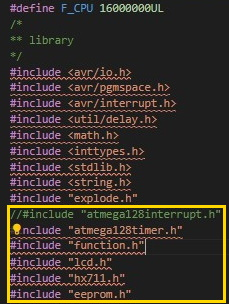
\includegraphics[scale=0.9]{./image/PESTA/Code/Livrarias.jpg}
	\caption{Livrarias}
	\label{Livrarias}
\end{figure}
\end{minipage}
\begin{minipage}{.6\linewidth}
Ao lado esta as livrarias usadas neste projeto, as que estão dentro da caixa amarela são as que foram criadas.
A filosofia usada é de criar objetos que representam o hardware para o poder manipular via código. Como se pode observar foi criado uma livraria para os temporizadores, outra paras as interrupções e \textbf{EEPROM} depois criado livrarias para os componentes externos, isto é, o \textbf{LCD} e o integrado \textbf{HX711}. \\
Uma abstração que torna simples executar qualquer algoritmo ou projeto, e isto só é possível depois de ultrapassar a barreira árdua e dolorosa de desenvolver as livrarias.
\\
\\
\\
\end{minipage}
\newpage
\section{Validação}
%%%To validate is to justify why the choices made and alternatives that could be chosen.
As escolhas feitas estão dentro dos parâmetros da oferta disponibilizada. Apenas o conhecimento adquirido ao aprofundar o funcionamento dos componentes é o ganho mais evidente, facilitando a interpretação de situações e deteção de anomalias (\textit{troubleshooting}), derivado aos custos dos materiais serem caros.\\
\\
Apostei na marca \textbf{Atmel} devido a experiência e conhecimentos já adquiridos, se aposta-se noutra marca teria de enfrentar uma curva de aprendizagem e adaptação que no final a nível de custos beneficio seria desfavorável, pelo tempo a dispensar e de ser muito trabalhoso a refazer tudo novamente noutra arquitetura.\\
\\
O sensor usado é o mais comum nesta pratica, e escolha demonstrada, o circuito de interface é indiferente a escolha apenas é baseada na sua precisão, ou seja, é de \textcolor{blue}{24} \textit{bit} enquanto o \textbf{ADC} do \textbf{MCU} de \textcolor{blue}{10} \textit{bit}.
\\
\\
\\
\subsection{Material}
Abaixo esta indicado uma tabela dos materiais usados, assim como os preços.
\\
\\
\begin{table}[H]{
		\caption{Lista de material}
		\rowcolors{3}{blue!80!yellow!50}{blue!70!yellow!40}
		\begin{tabular}{ |p{12cm}|c|p{2cm}|  }
			\hline
			\multicolumn{3}{|c|}{Lista de Material} \\
			\hline
			Peça & Quant & Preço [uni] \\
			\hline
			Fonte de alimetação 12V 1A & 1 & \EUR{3.87} \\
			Conversor DC-DC com voltímetro & 1 & \EUR{7.75} \\
			ET BASE AVR Atmega128 Board & 1 & \EUR{23.92} \\
			Test Input Board  & 1 & \EUR{3.71} \\
			Test Output Board & 1 & \EUR{3.71} \\
			IDC Socket 10 way    & 12 & \EUR{0.31} \\
			IDC Header Straight 10 way    & 12 & \EUR{0.25} \\
			Flatcable    & ? & \EUR{?} \\
			20x4 LCD Module Blue & 1 & \EUR{12.24} \\
			SparkFun Load Cell Amplifier HX711 & 1 & \EUR{13.04}   \\
			50Kg Load Cell & 1 & \EUR{12} \\
			\hline
			& \textit{total} & \EUR{86.96} \\
			\hline
		\end{tabular}
	}
	\label{material}
\end{table}


\subsection*{Testar}
Quanto a funcionalidade no seu todo a balança tem \textcolor{blue}{quatro} botões e \textcolor{blue}{três} \textit{leds} ativados, um botão para fazer o \textit{offset} no \textcolor{green}{PORTF 0}, e dois botões com dupla função, fazer \textit{reset} para \textit{default} e incrementar, outro para entrar no menu de calibração e decrementar, o \textcolor{blue}{quarto} botão é reservado para \textit{enter} e assumir o valor introduzido na calibração.\\
\\
O botão \textcolor{green}{PORTF 3} quando premido durante \textcolor{blue}{cinco} segundos faz um \textit{reset} para configuração \textit{default} depois de o \textit{led} no \textcolor{red}{PORTC 6} piscar \textcolor{blue}{quatro} vezes.\\
\\
O botão \textcolor{green}{PORTF 4} quando premido durante \textcolor{blue}{cinco} segundos entra no menu de calibração do valor do \textit{gain factor} e o \textit{led} no \textcolor{red}{PORTC 7} liga, usando os botões de incrementa e decrementar, isto é, o
\textcolor{green}{PORTF 3} e \textcolor{green}{PORTF 4} pode-se alterar esse valor.\\
\\
Para assumir o valor e sair do menu de calibração basta premir o botão colocado no \textcolor{green}{PORTF 5}. Tanto no caso de calibração ou de \textit{offset} os valores são guardados na \textbf{EEPROM} do microcontrolador, sendo que, se retirar a alimentação do circuito este não perde os valores e o \textit{led} \textcolor{red}{PORTC 5} permanece ligado.
\\
\\
%%%%%%%%%%%%%%%%%%%%%%%%%%%%%%%%%%%%%%%%%%%%%%%%%%%%%%%%%%%%%%%%
\begin{comment}
Sem contar com as despesas no equipamento para a programação do hardware que em principio só se gasta uma vez, isto é, se não se estragar. No caso do programador \textbf{Atmel-ICE} pode custar até \EUR{185.55}.\\
\\
É de ter em conta que os preços são \textbf{PVP}, que no caso se for preços comerciais são dez vezes inferior, e se for para produção em grande escala também tem descontos por quantidade.\\
$\begin{array}{l l l}
\text{Média} & & \\
\overline{x} & = & \frac{1}{n}\sum_{i=1}^n x_i
\end{array}$
MEMS devices and structures are fabricated using conventional integrated circuit process techniques, such as lithography, deposition, and etching, together with a broad range of specially developed micromachining techniques. \cite{book-9}
The three essential elements in conventional silicon processing are deposition, lithography, and etching. \cite{book-9}
Sensitivity,Long-Term Drift e Temperature Effects (Span temperature hysteresis).
\end{comment}
%%%%%%%%%%%%%%%%%%%%%%%%%%%%%%%%%%%%%%%%%%%%%%%%%%%%%%%%%%%%%%%%